%-------------------------------------------------
%
% Time.tex
%
%------------------------------------------------
\section[Tempi di risoluzione]{tempi di risoluzione}
\label{pt2:time}
Le esecuzioni dell'algoritmo genetico si sono svolte prendendo in considerazione le medesime istanze utilizzate per la prima parte del progetto e per ogni singola istanza si sono eseguiti 10 \english{test} indipendenti. Per ogni esecuzione si è registrato il tempo di risoluzione ed il valore della funzione obiettivo.

L'algoritmo si è eseguito generando, di volta in volta, una popolazione di 200 individui ed eseguendo 50 evoluzioni genetiche.

Si sono ottenuti i risultati riportati nelle Tabelle 2.3 2.4 2.5.

\begin{table}[htbp]
\centering
\label{pt1:time:tabular_random}
\begin{tabular}{|c|c|c|c|}
\hline
\multicolumn{3}{|c|}{Random}\\
\hline
\textbf{Classe} & \textbf{Media (ms))} & \textbf{Media (hh:mm:ss:mmm)}\\
\hline
5   &   9519 & 00:00:09:519\\
\hline
10  &  17053 & 00:00:17:053\\
\hline
15  &  16602 & 00:00:16:602\\
\hline
20  &  21157 & 00:00:21:157\\
\hline
30  &  32085 & 00:00:32:085\\
\hline
40  &  35339 & 00:00:35:339\\
\hline
50  &  38044 & 00:00:38:044\\
\hline
60  &  42798 & 00:00:42:798\\
\hline
70  &  54999 & 00:00:54:999\\
\hline
80  &  70692 & 00:01:10:692\\
\hline
90  &  63203 & 00:01:03:203\\
\hline
100 &  66344 & 00:01:06:344\\
\hline
\end{tabular}
\caption{Tempi medi di esecuzione classe random}
\end{table}

\begin{table}[htbp]
\centering
\label{pt1:time:tabular_random}
\begin{tabular}{|c|c|c|c|}
\hline
\multicolumn{3}{|c|}{Cluster}\\
\hline
\textbf{Classe} & \textbf{Media (ms))} & \textbf{Media (hh:mm:ss:mmm)}\\
\hline
5   &   9127 & 00:00:09:127\\
\hline
10  &  16251 & 00:00:16:251\\
\hline
15  &  15901 & 00:00:15:901\\
\hline
20  &  21785 & 00:00:21:785\\
\hline
30  &  32877 & 00:00:32:877\\
\hline
40  &  34928 & 00:00:34:928\\
\hline
50  &  40173 & 00:00:40:173\\
\hline
60  &  46305 & 00:00:46:305\\
\hline
70  &  55937 & 00:00:55:937\\
\hline
80  &  61289 & 00:01:01:289\\
\hline
90  &  66961 & 00:01:06:961\\
\hline
100 &  72772 & 00:01:12:772\\
\hline
\end{tabular}
\caption{Tempi medi di esecuzione classe cluster}
\end{table}

\begin{table}[htbp]
\centering
\label{pt1:time:tabular_random}
\begin{tabular}{|c|c|c|c|}
\hline
\multicolumn{3}{|c|}{circle}\\
\hline
\textbf{Classe} & \textbf{Media (ms))} & \textbf{Media (hh:mm:ss:mmm)}\\
\hline
5   &   8974 & 00:00:08:974\\
\hline
10  &  16781 & 00:00:16:781\\
\hline
15  &  16603 & 00:00:16:603\\
\hline
20  &  24290 & 00:00:24:290\\
\hline
30  &  36473 & 00:00:36:473\\
\hline
40  &  41144 & 00:00:41:144\\
\hline
50  &  46978 & 00:00:46:978\\
\hline
60  &  51585 & 00:00:51:585\\
\hline
70  &  68114 & 00:00:68:114\\
\hline
80  &  70622 & 00:01:10:622\\
\hline
90  &  64841 & 00:01:04:841\\
\hline
100 &  70179 & 00:01:10:179\\
\hline
\end{tabular}
\caption{Tempi medi di esecuzione classe circle}
\end{table}

\begin{figure}
\centering
\begin{subfigure}[b]{0.9\textwidth}
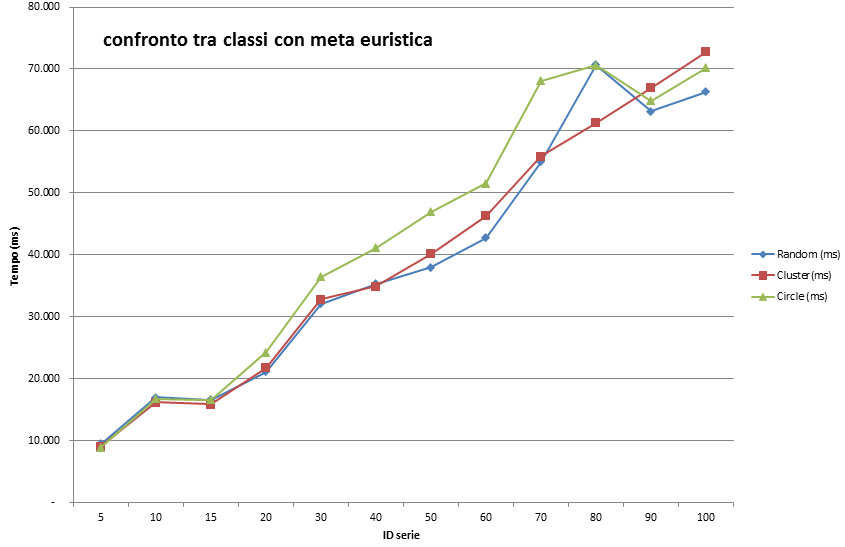
\includegraphics[width=\textwidth]{Images/Part_2/graphics/Times01.png}
\caption{Tempi di risoluzione al variare dei punti}
\label{pt2:time:time01}
\end{subfigure}

\begin{subfigure}[b]{0.9\textwidth}
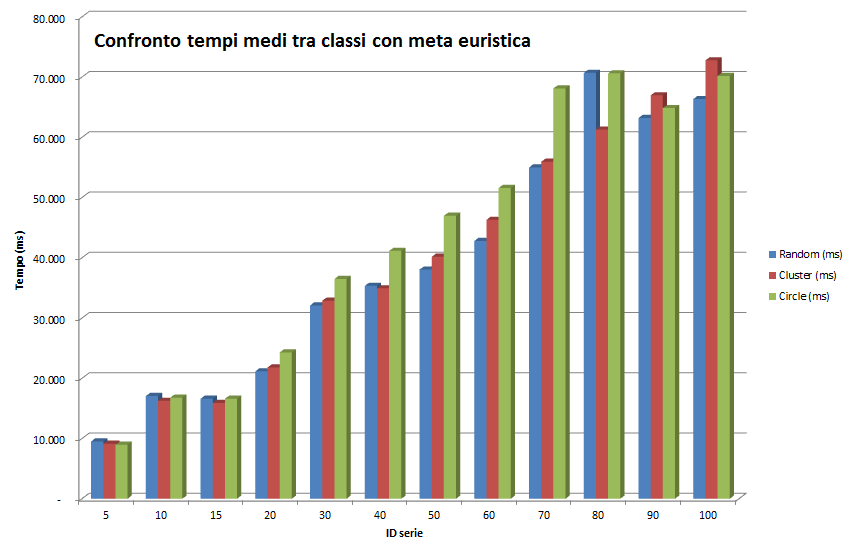
\includegraphics[width=\textwidth]{Images/Part_2/graphics/Times02.png}
\caption{Tempi di esecuzione per tipologia}
\label{pt2:time:time02}
\end{subfigure}
\caption{Confronto tempistiche}
\label{pt1:time:times}
\end{figure}

\subsection[Conclusioni]{conclusioni}
\label{pt2:time:conclusion}
L'utilizzo di una metaeuristica porta un notevole vantaggio, rispetto all'utilizzo di un algoritmo esatto, dal punto di vista del tempo di computazione.

A differenza di un algoritmo esatto, come si evince dai grafici in Figura 2.1, il tempo di computazione rimane stabile al variare della distribuzione di punti, e vi è una crescita lineare rispetto all'esponenzialità dell'algoritmo esatto.

Occorre però riflettere sulla precisione del risultato ottenuto. All'aumentare del numero di punti la differenza tra la soluzione esatta e la media ritornata dalla meta euristica è notevole, però con un analisi più attenta dei parametri che compongono l'algoritmo sono sicuro si potrebbero ottenere un aumento della precisione, riducendo cosi la differenza dal valore ottimo.

Alcuni miglioramenti all'algoritmo genetico possono essere:

\begin{itemize}
\item introduzione di fasi di diversificazione per evitare che la popolazione possa convergere prematuramente verso quello che potrebbe essere un massimo/minimo locale;
\item far evolvere un figlio, prima della creazione di una nuova generazione, attraverso algoritmi di ricerca locale;
\end{itemize}